% !TeX root = ../main.tex
% Add the above to each chapter to make compiling the PDF easier in some editors.

\chapter{Discussion}\label{chapter:discussion}

In this chapter the choice of learning schemes is discussed as well as the performance of the neural networks trained accordingly is evaluated. The reward functions are analysed and their impact on training and testing performance is measured.

\section{Training Performance}
As mentioned in Section \ref{snnRL}, the classical reinforcement learning approach based on MDP is not directly applicable to asynchronous spike trains in continuous time. Adapted algorithms relying on actor-critic network architecture and place cells as state space representation have been shown to work well for relatively small state spaces (a 5\(\times\)5 grid-world, \cite{18}, \cite{19}, \cite{21}) but they fail for high-dimensional tasks. \\
Reward-modulated STDP learning rules as discussed in Section \ref{armmrm} provide biologically inspired reinforcement learning framework based on dopaminergic facilitation or depression of synapses, modifying their plasticity. In this work, additive reward-modulated STDP and multiplicative reward-modulated STDP learning rules were used to train a neural network to control snake-like robot navigating in an environment closed by walls. The training model developed in this paper focuses on an agent that only relies on sensory input, without any critic or model information. As described in Sections \ref{sectionDVStoSNN} and \ref{rewardSig} the reward function is chosen in such a way, that the signal it produces correlates directly with the DVS input to SNN. With neuromodulator baseline of 0 the networks strives to minimize its reward to 0, which reflects the desired behaviour of staying in the center of an enclosed space. 

\subsection{ARM-STDP with center-approximating reward function}

The most simple training model proposed is the ARM-STDP learning rule with center-approximating reward function as specified in \eqref{eq:centerReward}. The reward function has some drawbacks, which can potentially break the training or testing sequences. In particular, if snake moves directly at the wall, the distance approximation would be roughly the same on both sides, leading to reward signal vanishingly small. This will mean, that the snake will travel in a straight line until it hits the wall. Another drawback is that if the snake moves into a turn while being close to the inner turning wall, the reward signal would be incorrect in a sense, that it would induce the snake to turn away from the inner wall and depending on how narrow the turn is, it will potentially lead to the snake unable to avoid collision in time.
The training sequence was completed in 5700 simulation steps with 2 collisions in the beginning of the right U-Turn, at the step 180 and in the middle of the left U-Turn, at the step 2603. In Fig. \ref{fig:trainingReward} the reward development through time is plotted. The moment of collision can be seen as extreme dips on the plot. In Fig. \ref{fig:armcenterweight} the development of weights during the training is plotted with weights of synapses connected to the left motor on top and to the right motor on the bottom. One can see that the shapes of left and right weights change are mimicking each other. The collision observed in episodes 180 and 2603 can see inducing significant changes, that stabilize afterwards.

\begin{figure}[h]
	\centering
	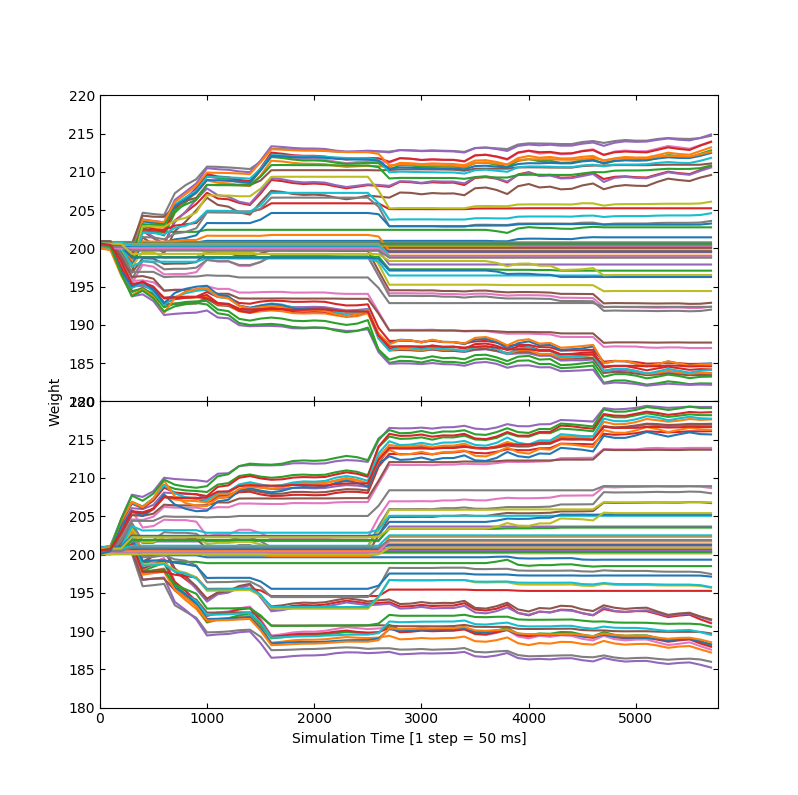
\includegraphics[scale=0.8]{ARMCENTERWEIGHTS.png}
	\caption{Weights development of ARM-STDP with center approximating reward function over simulation time}\label{fig:armcenterweight}
\end{figure}
\begin{figure}[h]
	\centering
	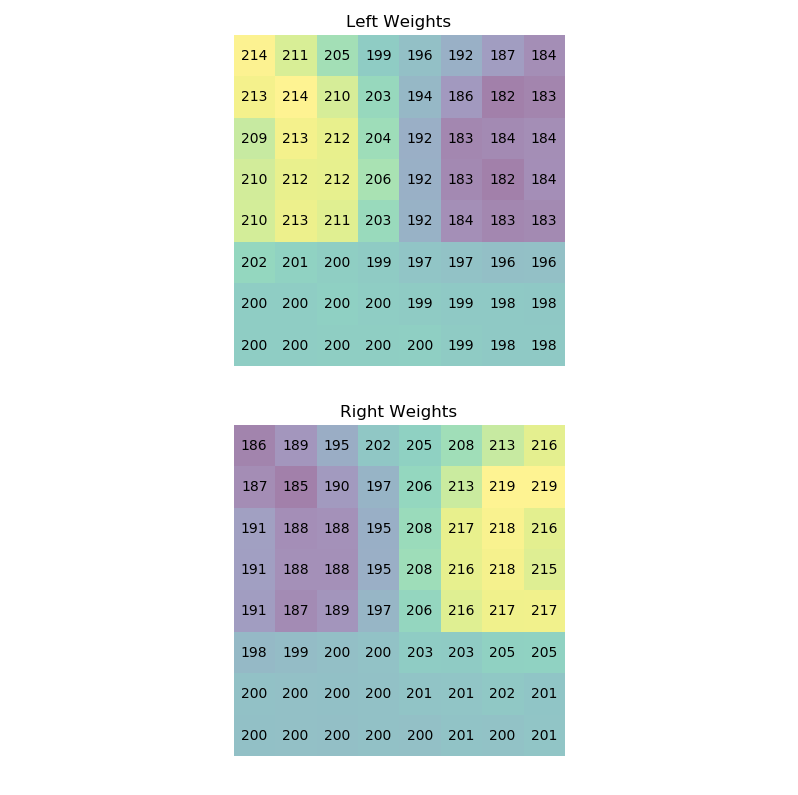
\includegraphics[scale=0.8]{ARMCENTERTESTWEIGHTS.png}
	\caption{Final weight distribution of ARM-STDP with center approximating reward function over simulation time}\label{fig:armcentertestweight}
\end{figure}

In Fig. \ref{fig:armcentertestweight} it is noticeable, that the weights reflect a DVS simulation frame, with left and right wall shapes mirrored in weights distribution.

\subsection{ARM-STDP with triangle area reward function}
In order to improve on the drawbacks of the simple center approximation function an area-based function is proposed as specified in Section \ref{rewardSig}. While the movement straight at the wall still is unresolved, the slithering gait induces the area changes to produce a slight turning behaviour before impact. The second drawback however is mitigated by the fact, that this reward function uses all 5 proximity sensors to produce a well distributed reward signal. In Fig. \ref{fig:trainingReward}, \ref{fig:armareaweight}, \ref{fig:armareatestweight} the reward during testing, weights evolution and final weight distribution are plotted. The training sequence was complete in 5400 steps with 2 collisions in left and right U-Turn stage at step 487 and 2187.

\begin{figure}[h]
	\centering
	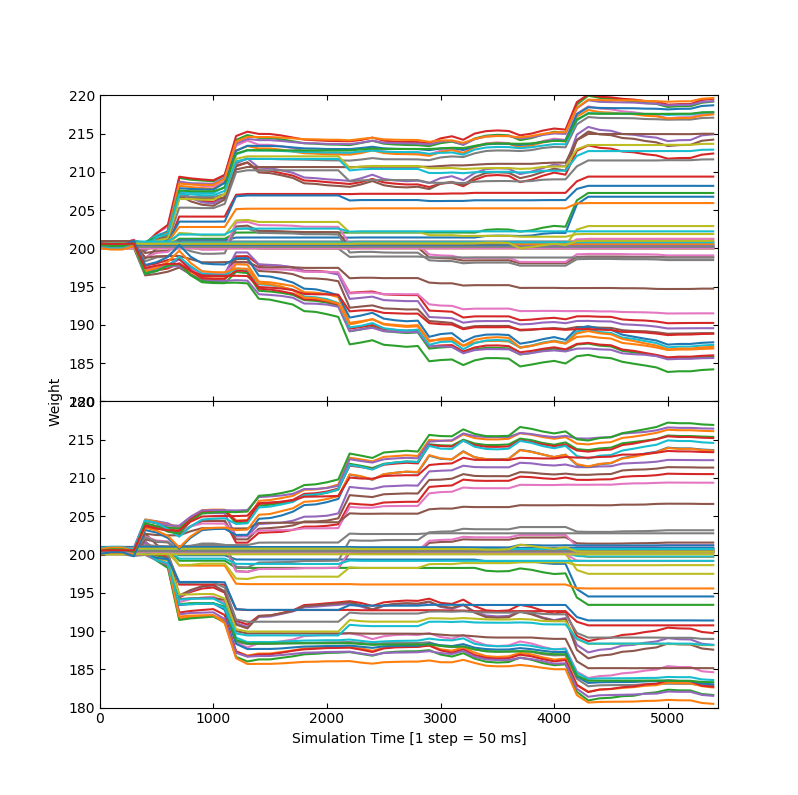
\includegraphics[scale=0.8]{ARMAREAWEIGHTS.png}
	\caption{Weights development of ARM-STDP with area-based approximating reward function over simulation time}\label{fig:armareaweight}
\end{figure}
\begin{figure}[h]
	\centering
	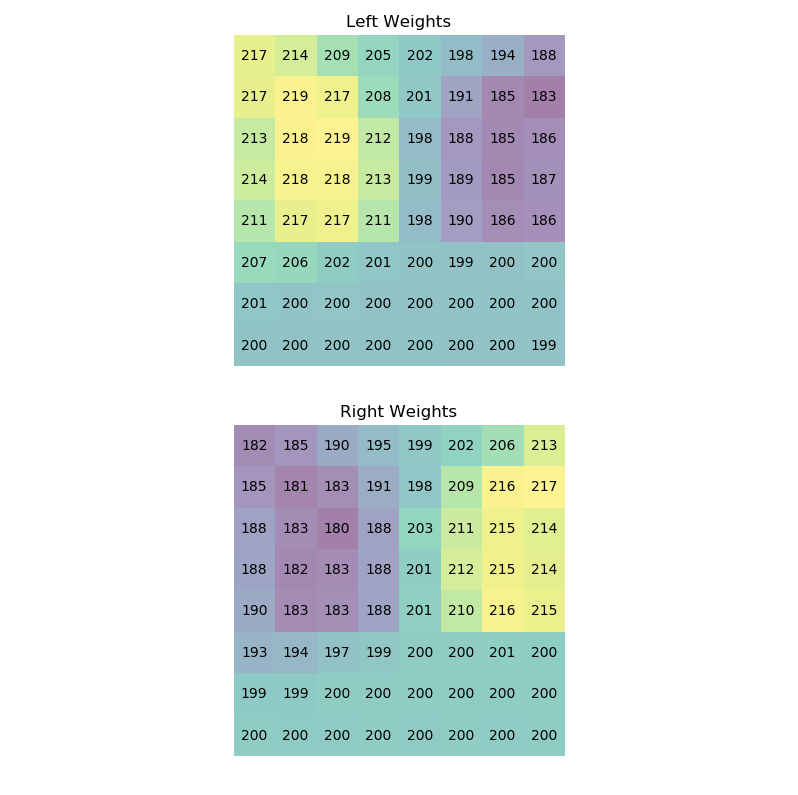
\includegraphics[scale=0.8]{ARMAREATESTWEIGHTS.png}
	\caption{Final weight distribution of ARM-STDP with area-based approximating reward function over simulation time}\label{fig:armareatestweight}
\end{figure}

\subsection{MRM-STDP with center-approximating reward function}

Multiplicative reward modulation behaves differently compared to additive as described in \cite{16}. It produces weight distributions that are more stable under input distortion. Weights also reach their final form quicker. Here, the training results for MRM-STDP with center-approximating and area-based reward function are shown. From the plots, it is obvious that the weights do indeed reach its stable distribution much quicker and the reward signal form reflects that as well. The MRM-STDP with center-approximating function finished training sequence in 4900 steps with 2 collisions at step 210 and 770, while the area-based variant finished in 4800 steps and 1 collision at step 771. (See Fig. \ref{fig:trainingReward}, \ref{fig:mrmcenterweight}, \ref{fig:mrmcentertestweight}, \ref{fig:mrmareaweight}, \ref{fig:mrmareatestweight})

\begin{figure}[h]
	\centering
	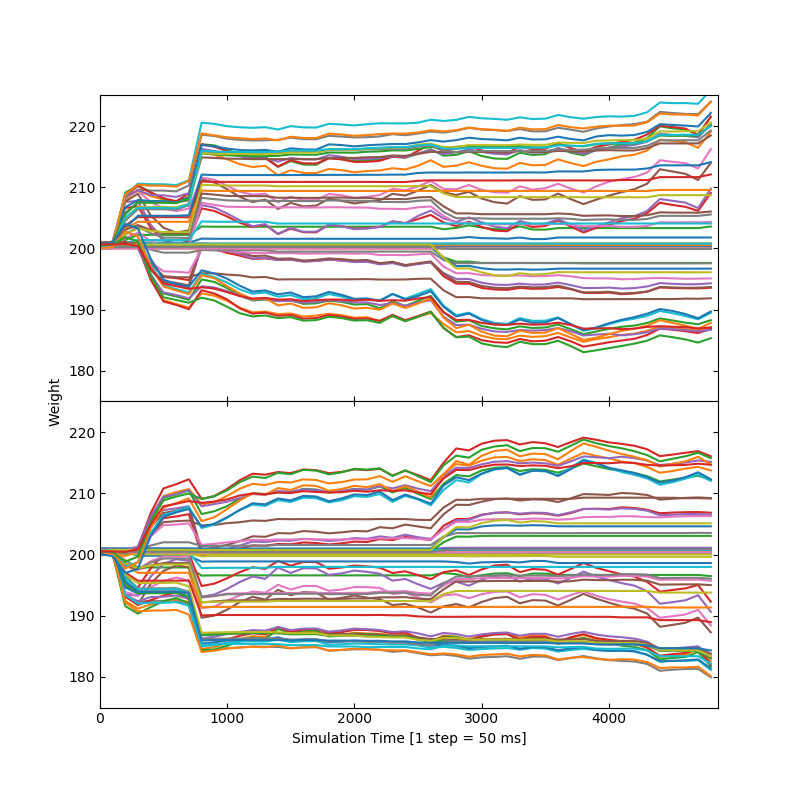
\includegraphics[scale=0.8]{MRMCENTERWEIGHTS.png}
	\caption{Weights development of MRM-STDP with center-approximating approximating reward function over simulation time}\label{fig:mrmcenterweight}
\end{figure}
\begin{figure}[h]
	\centering
	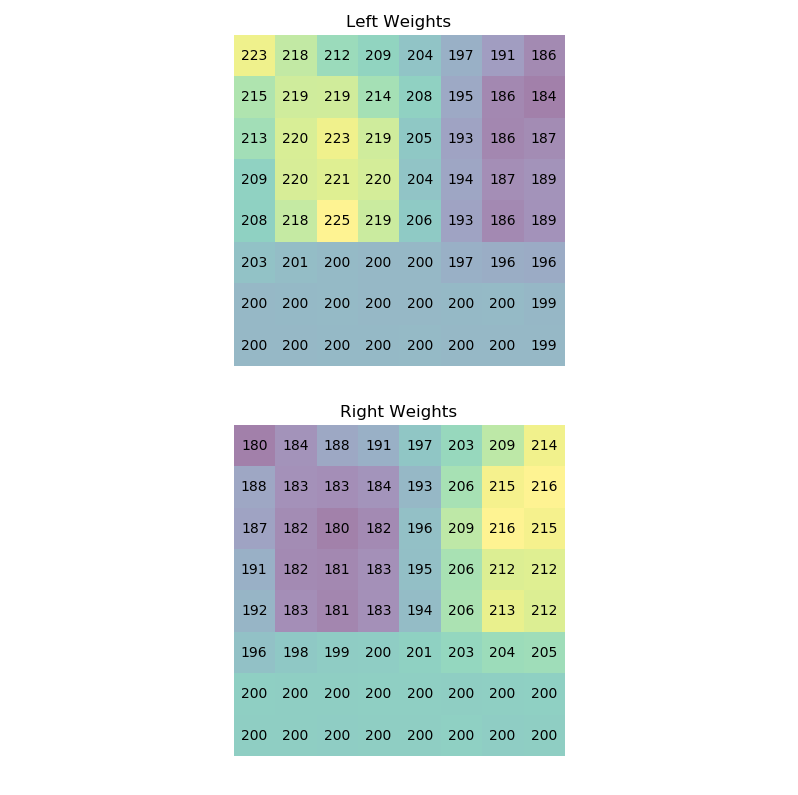
\includegraphics[scale=0.8]{MRMCENTERTESTWEIGHTS.png}
	\caption{Final weight distribution of MRM-STDP with center-approximating approximating reward function over simulation time}\label{fig:mrmcentertestweight}
\end{figure}


\begin{figure}[h]
	\centering
	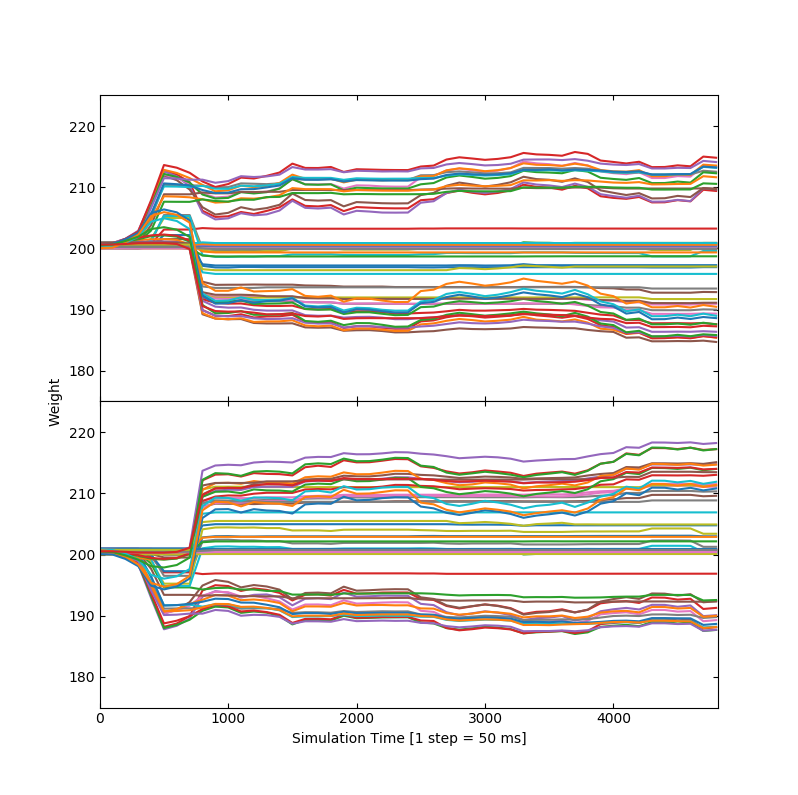
\includegraphics[scale=0.8]{MRMAREAWEIGHTS.png}
	\caption{Weights development of MRM-STDP with area-based approximating reward function over simulation time}\label{fig:mrmareaweight}
\end{figure}
\begin{figure}[h]
	\centering
	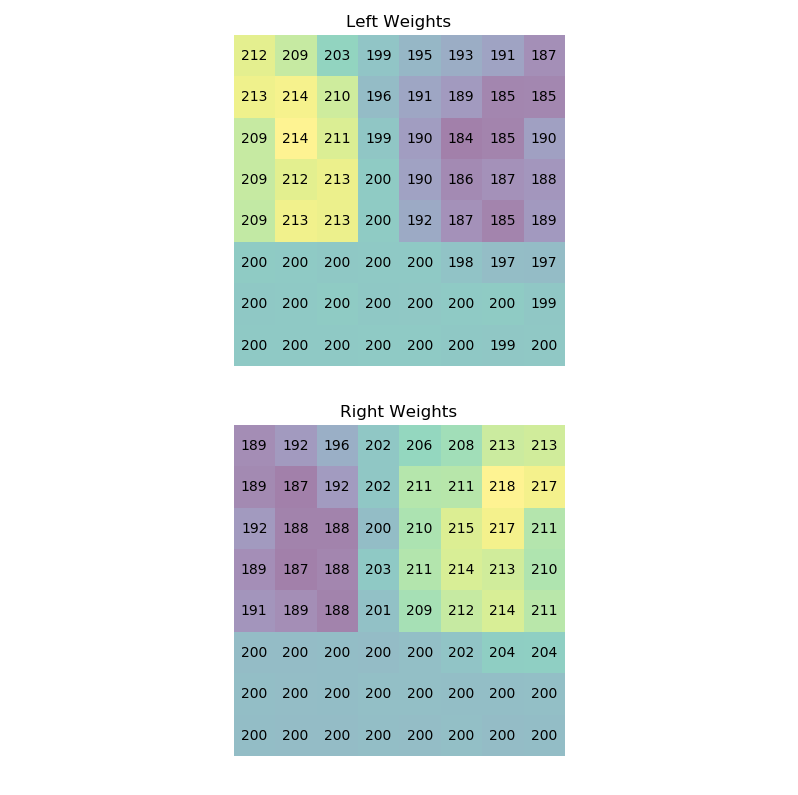
\includegraphics[scale=0.8]{MRMAREATESTWEIGHTS.png}
	\caption{Final weight distribution of MRM-STDP with area-based approximating reward function over simulation time}\label{fig:mrmareatestweight}
\end{figure}

\section{Testing Performance}

The 4 variants of trained SNNs were tested on adaptiveness in a second V-REP scenario. All 4 conrollers were able to complete test scenario on the first try. Subsequently each controller was run for 50000 steps on a testing scenario, while logging instantaneous reward, distance traveled, each collision as fail and each completed lap as success. Each controller was able to navigate the testing scenario without fail, running on average 1188.4 meters or ~27 laps.

\begin{figure*}[t!]
	\centering
	\begin{subfigure}{0.5\textwidth}
		\centering
		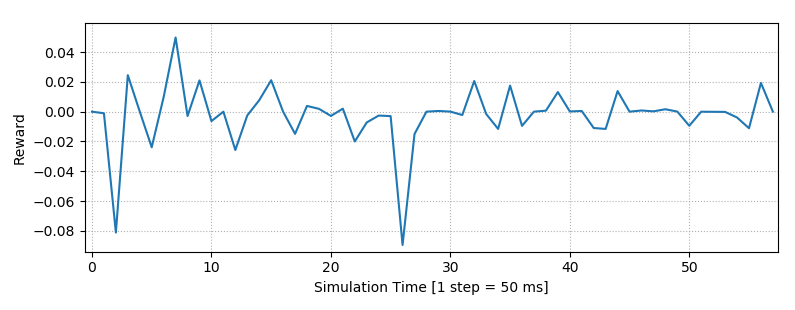
\includegraphics[scale=0.5]{ARMCENTERREWARD.png} 
		\caption{}
	\end{subfigure}\\
	\begin{subfigure}{0.5\textwidth}
		\centering	
		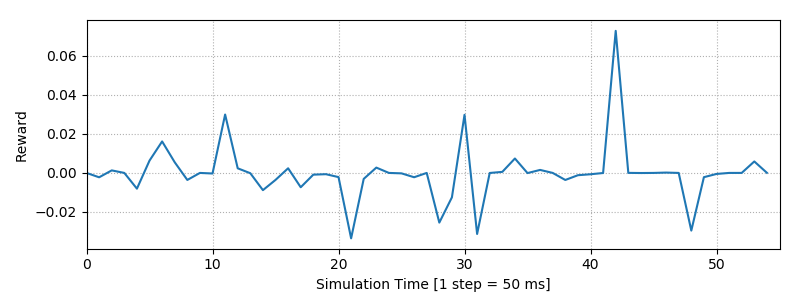
\includegraphics[scale=0.5]{ARMAREAREWARD.png}
		\caption{}
	\end{subfigure}
	\begin{subfigure}{0.5\textwidth}
		\centering	
		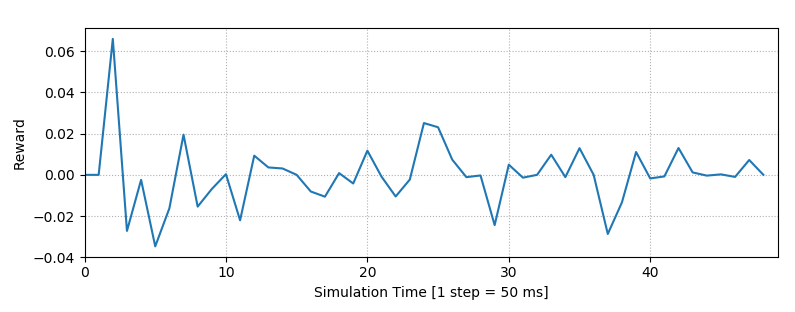
\includegraphics[scale=0.5]{MRMCENTERREWARD.png}
		\caption{}
	\end{subfigure}
	\begin{subfigure}{0.5\textwidth}
		\centering
		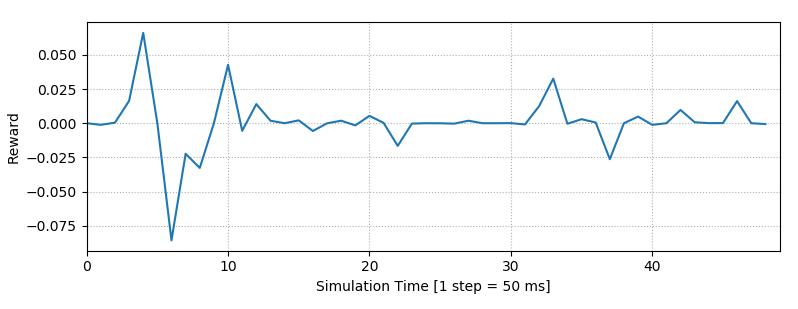
\includegraphics[scale=0.5]{MRMAREAREWARD.png}
		\caption{}
	\end{subfigure}
	\caption{Reward signals: (a) - ARM-STDP center-approximating, (b) - ARM-STDP area-based, (c) - MRM-STDP, center-approximating, (d) - MRM-STDP area-based}\label{fig:trainingReward}
	
\end{figure*}

\subsection{Performance Summary}

It proved to be difficult to define a sane metric to compare testing performance, since the robot's task was to advance in a wall-enclosed environment without collisions. Each controller was able to complete 50000 simulation steps without encountering a collision. However in training performance, the multiplicative rule shows clear advantages in learning speed. It completes the training sequence on average quicker then additive rule based network as well as reaches stable weight distribution faster. Training data also seems to suggest, that an area-based reward function behaves more stable then center approximation based function. 